\chapter{Méthodologie et Cycle de Vie}

\section{Approche Agile (Scrum)}

Face à un projet comportant une forte incertitude technique (technologies nouvelles, architecture distribuée), nous avons opté pour une approche Agile. Plutôt que de livrer tout à la fin, nous avons procédé par itérations courtes (Sprints).

À la fin de chaque Sprint, une phase de validation (Recette) a permis à la MOA de vérifier que le flux de données correspondait aux attentes (ex: vérification des événements dans le producteur Kafka).

\section{Utilisation de Taiga (Kanban)}

Pour gérer le flux de travail au quotidien, nous avons mis en place un tableau Kanban sur la plateforme Taiga.

\begin{borderedfigure}
    \centering
    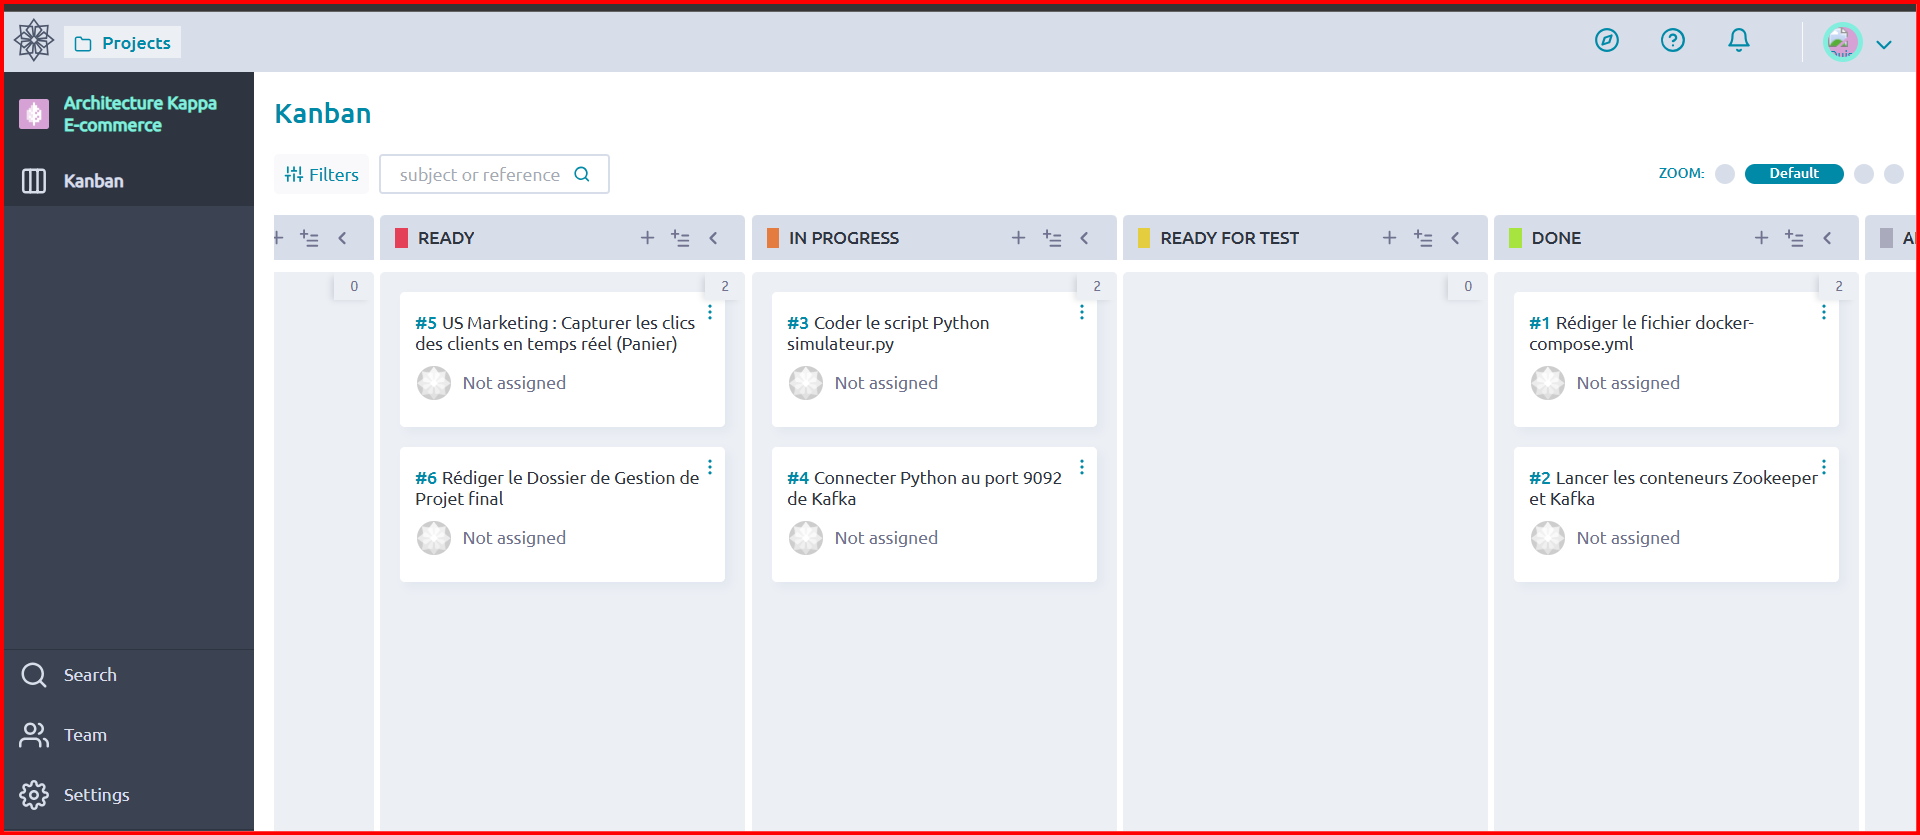
\includegraphics[width=\textwidth]{../screenshots/taiga.png}
    \captionof{figure}{Tableau Kanban du projet sur Taiga}
\end{borderedfigure}

Cet outil nous a permis de visualiser les User Stories (US), de suivre leur état d'avancement (Ready, In Progress, Done) et d'assurer une bonne communication au sein de l'équipe projet.
